\section{Introduccion a la Metodologia Lean}

\subsection{Orignes de Lean}

En una primera instancia la produccion era artesanal, luego comenzo a ser en masa para terminar siendo una produccion en sistema o system production.

Luego de la segunda guerra mundial, Toyota se vio obligada a adaptarse a un mercado que no le permitia producir en masa, por lo que se vio obligada a producir bajo demanda. Para ello, se implemento el sistema Just in Time (JIT), que es la base de la metodologia Lean.

\begin{figure}[H]
\centering
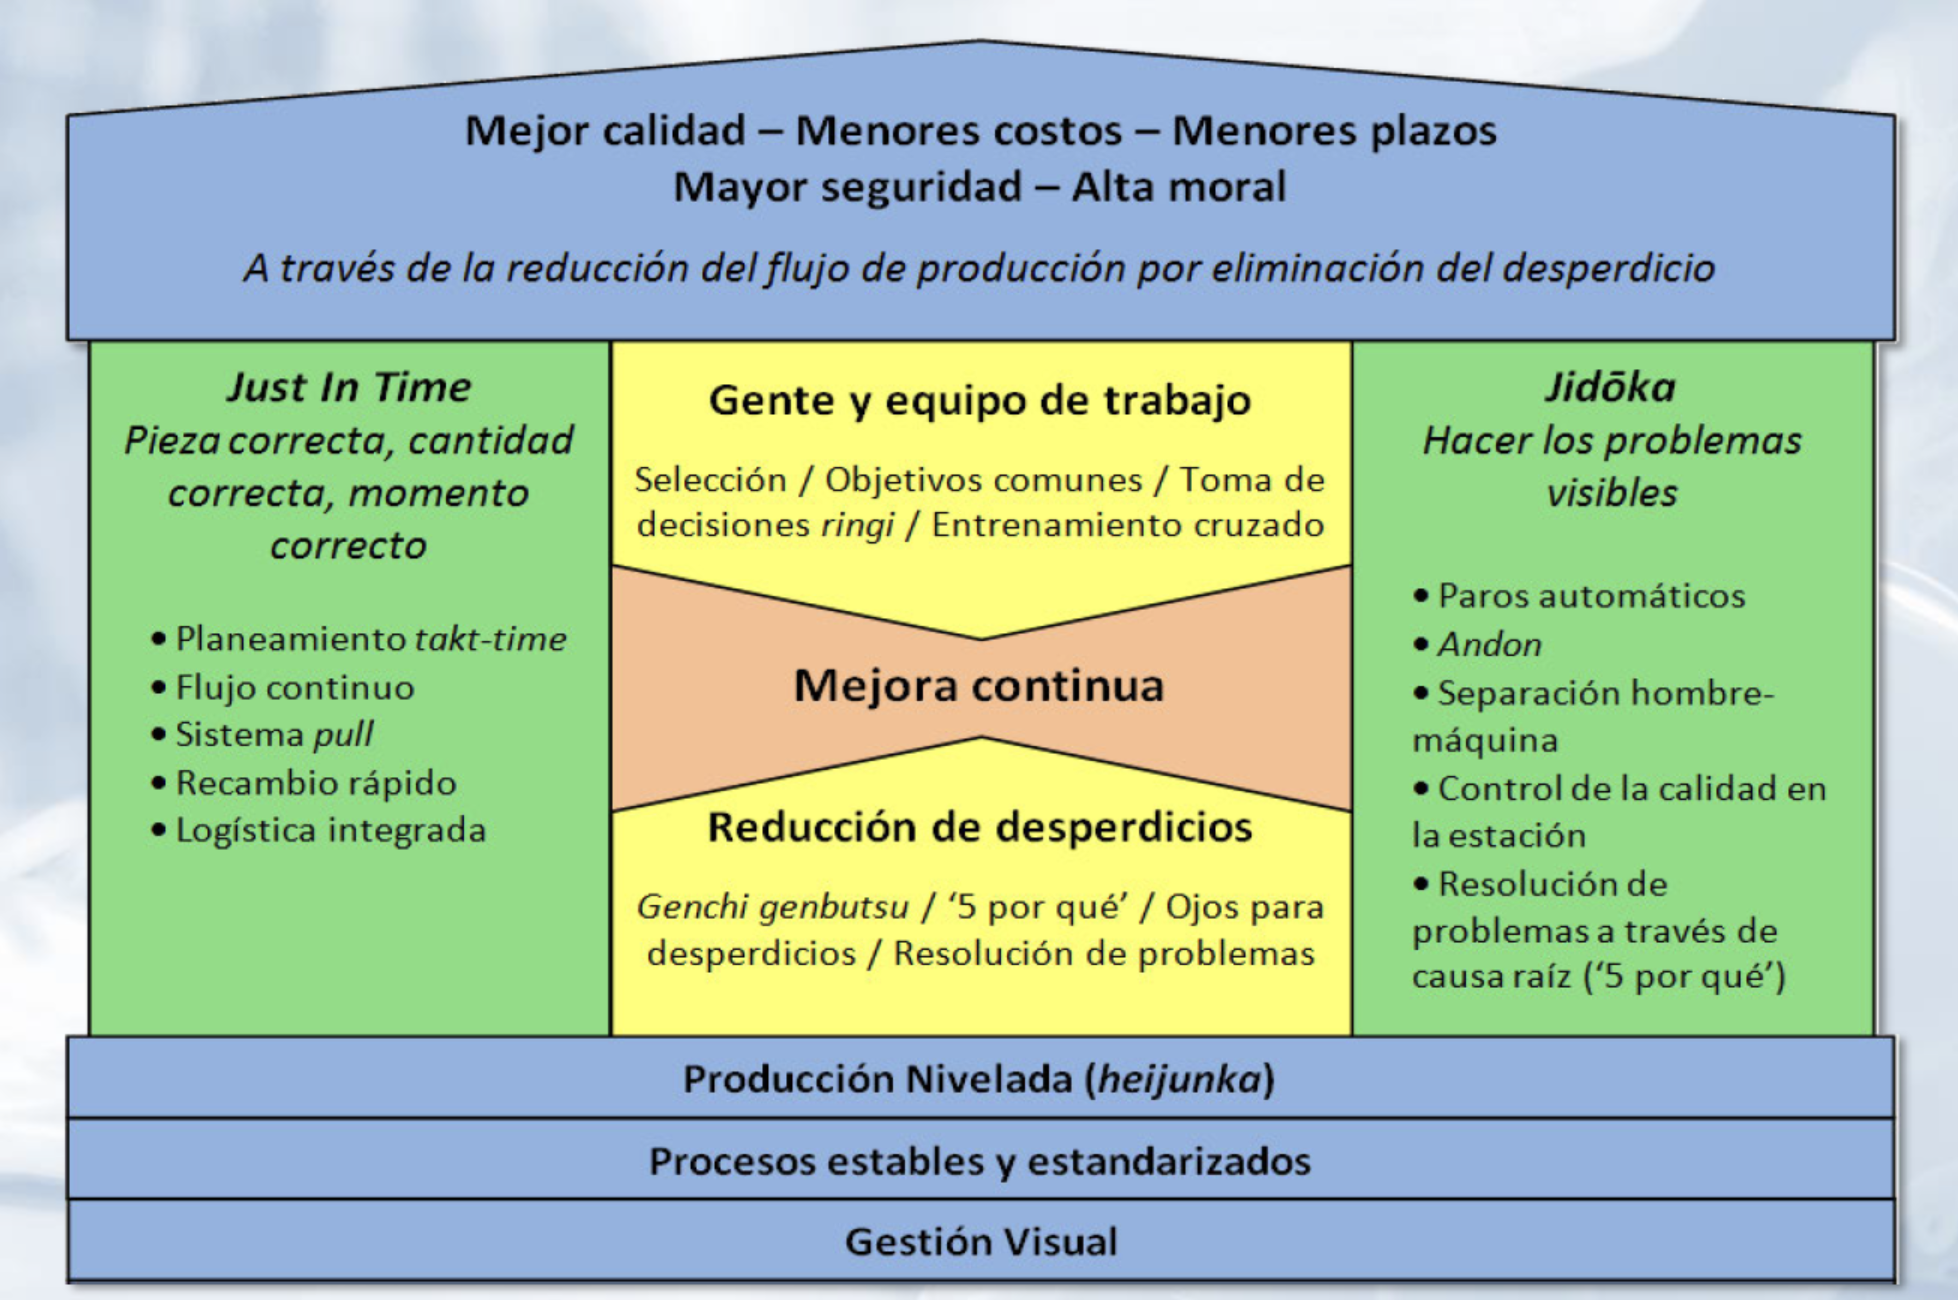
\includegraphics[width=0.8\textwidth]{IMAGENES/toyota.png}
\caption{Toyota y el origen de Lean}
\label{fig:lean}
\end{figure}

Por lo tanto, que es LEAN?

Lean busca \textbf{maximizar el valor} del producto, \textbf{minimizando el desperdicio}.

\begin{itemize}
    \item Es útil para mejorar cualquier proceso en cualquier organización
    \item Es una filosofía, una forma de ver, pensar y actuar
    \item No entrega soluciones inmediatas
\end{itemize}

\subsection{Principios de Lean}

\begin{enumerate}
    \item Especificar el valor
    \item Identificar el flujo de valor
    \item Hacer fluir el valor
    \item Pull del valor
    \item Buscar la perfección
\end{enumerate}

\subsubsection{Especificar el valor}

Se buscan \textbf{productos especificos} con \textbf{capacidades especificas} que satisfacen las necesidades de los \textbf{clientes especificos} a \textbf{precios especificos}.

\subsubsection{Identificar el flujo de valor}

Son las acciones especificas para crear un producto, desde la materia prima hasta el cliente final.

\begin{figure}[H]
\centering
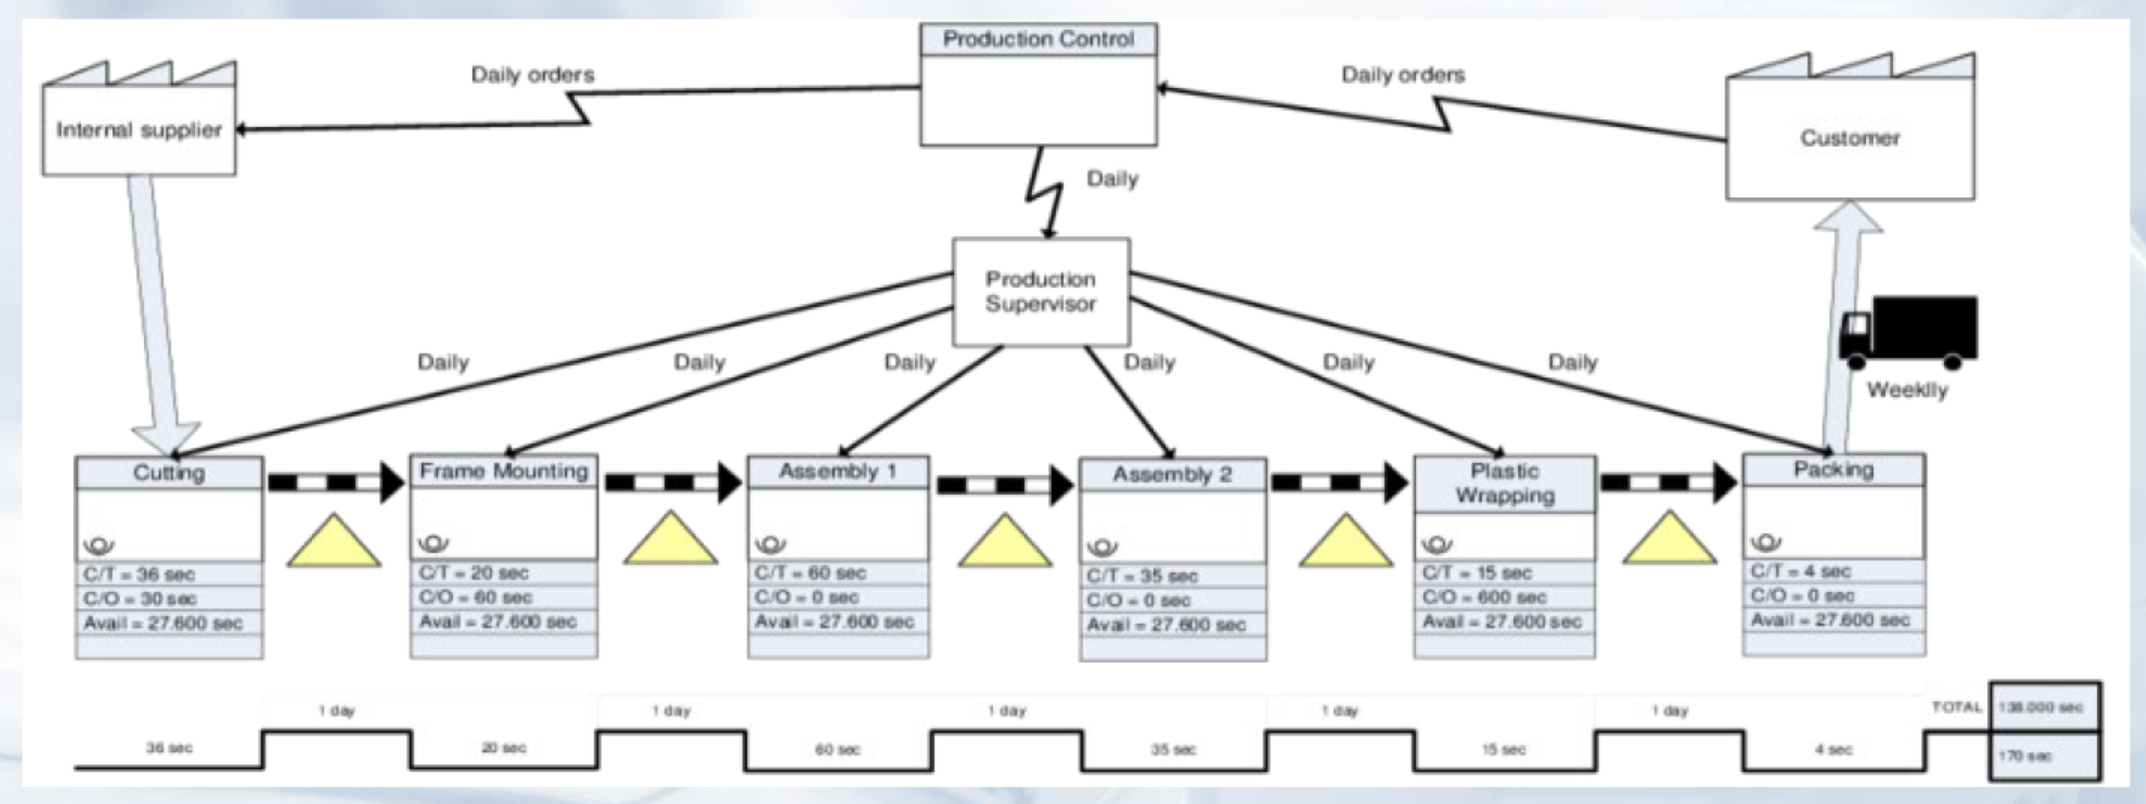
\includegraphics[width=0.8\textwidth]{IMAGENES/flujo.png}
\caption{Flujo de valor}
\label{fig:flujo_valor}
\end{figure}

\subsection{Hacer fluir el valor}

Enfocarse en el producto y sus nesecidades, mas que en la maquinaria

\begin{figure}[H]
\centering
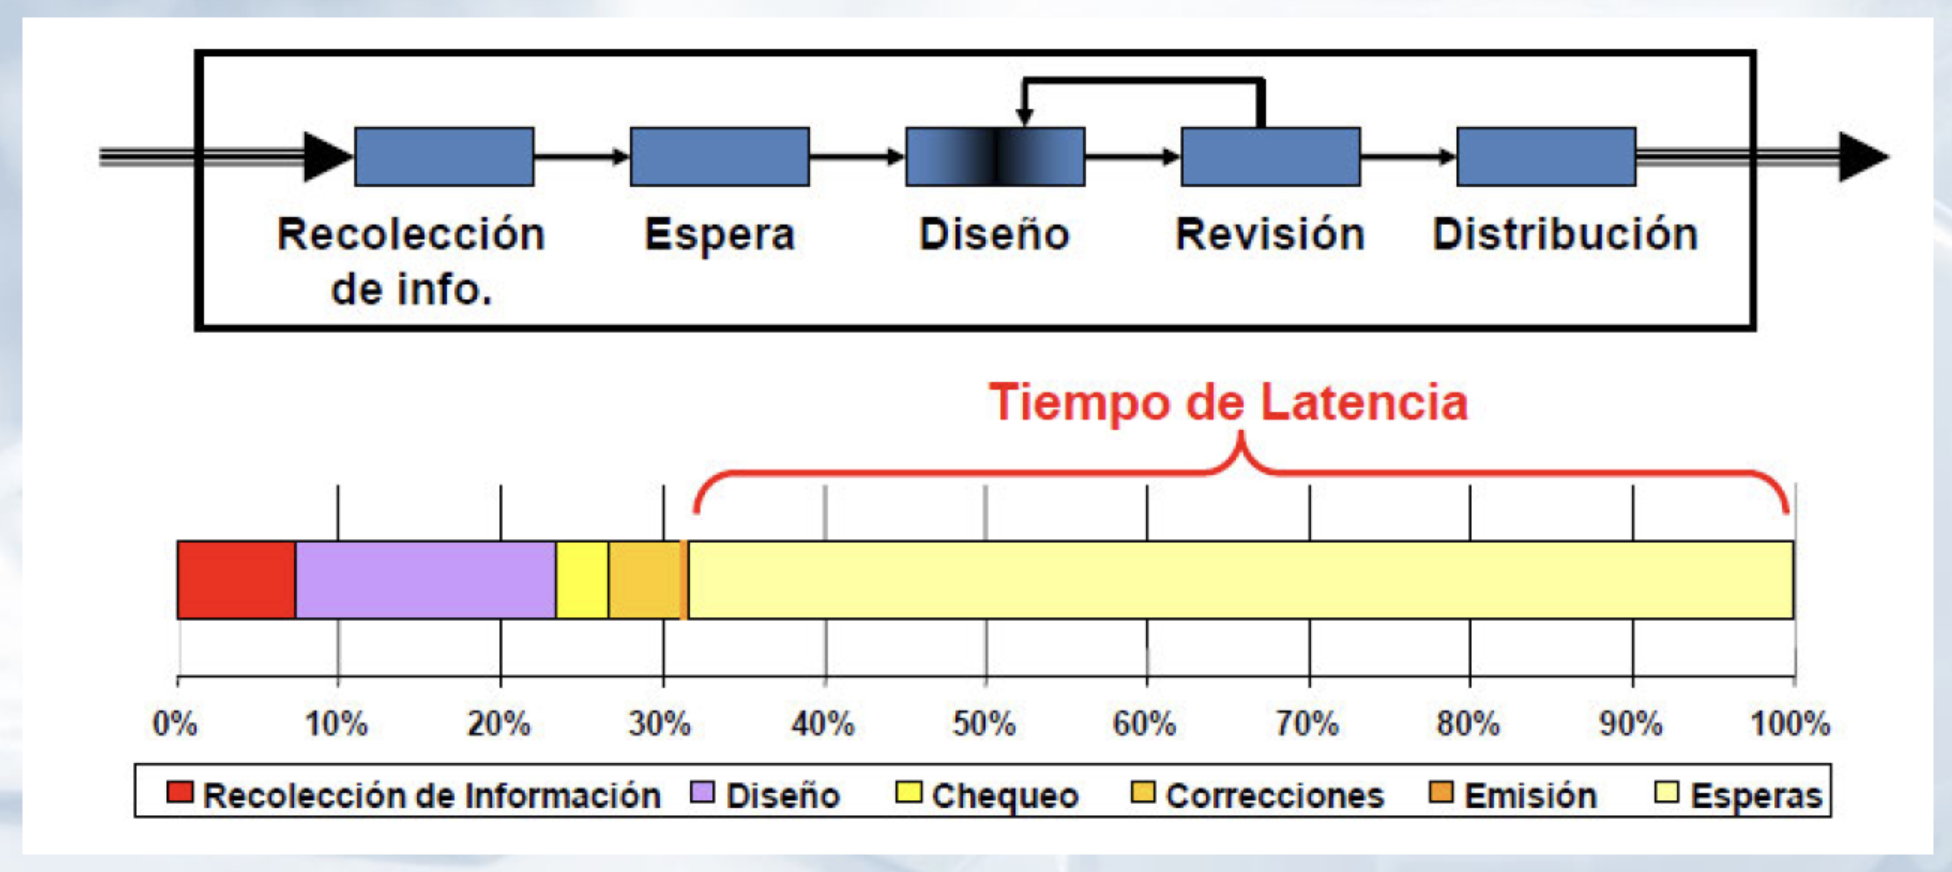
\includegraphics[width=0.8\textwidth]{IMAGENES/fluir.png}
\caption{Hacer fluir el valor}
\label{fig:flujo_valor}
\end{figure}

\subsection{Pull del valor}

Nadie aguas arriba produce algo que no se le ha pedido, y nadie aguas abajo recibe algo que no ha solicitado.

\subsection{Buscar la perfección}

Todos deben poder ver y ser parte del proceso, y todos deben poder contribuir a la mejora continua.

\subsection{Cambio del Pensamiento}

\begin{table}[H]
\centering
\begin{tabularx}{\textwidth}{|l|X|X|X|}
\hline
\textbf{} & \textbf{ARTESANAL} & \textbf{PRODUCCIÓN MASIVA} & \textbf{PENSAMIENTO LEAN} \\
\hline
\textbf{Focalización} & Tarea & Producto & Cliente \\
\hline
\textbf{Operación} & Ítems individuales & Lote y cola & Flujo y pull sincronizado \\
\hline
\textbf{Objetivo general} & Dominio de la actividad & Reducir costos y aumentar eficiencia & Eliminar desechos y agregar valor \\
\hline
\textbf{Calidad} & Integración (parte de la actividad) & Inspección (una segunda etapa después de producción) & Inclusión (incorporada por diseño y métodos) \\
\hline
\textbf{Estrategia de negocio} & Personalización & Economías de escala y automatización & Flexibilidad y adaptabilidad \\
\hline
\textbf{Mejoramiento} & Mejoramiento continuo determinado por un maestro & Mejoramiento periódico determinado por experto & Mejoramiento continuo determinado por trabajador \\
\hline
\end{tabularx}
\caption{Comparación entre modelos de producción: artesanal, masiva y pensamiento Lean}
\end{table}

Adicionalmente, se genero un cambio en el pensamiento del costo.

Tradicionalmente

\begin{equation}
    \text{Precio} = \text{Costo} + \text{Margen de ganancia}
\end{equation}

En cambio, en Lean

\begin{equation}
    \text{Margen de Ganancia} = \text{Precio} - \text{Costo}
\end{equation}

Para que sea exitoso, \textbf{todos} deben estar involucrados en la cadena de valor.

\subsection{Beneficios de Lean}

\begin{itemize}
    \item Los tiempos totales de producción \textbf{disminuyen un 90\%}
    \item Las existencias se \textbf{reducen también un 90\%}
    \item Los defectos se \textbf{reducen en un 50\%}
    \item El plazo de entrega se \textbf{reduce en un 50\%}
\end{itemize}
